\documentclass{beamer}

\usepackage[utf8]{inputenc}
%\usepackage[scaled]{uarial} % not available in Linux
\renewcommand{\rmdefault}{phv} % Arial

\renewcommand{\sfdefault}{phv} % Arial
\renewcommand*\familydefault{\sfdefault} %% Only if the base font of the document is to be sans serif

\usepackage[T1]{fontenc}
\usepackage{classico}
\usepackage{siunitx}

\title{Classificazione dei bosoni elettrodeboli con una rete neurale al Large Hadron Collider} 
\subtitle{6 Novembre 2024}
\date{6 Novembre 2024}
\author{Jacopo Lancione}

\usetheme{UNITO}
    %\setbeamercovered{invisible} %default
    \setbeamercovered{transparent} % Items to be uncovered already visible, but almost transparent
    
\begin{document}
\begin{frame}
    \titlepage
\end{frame}

\begin{frame}{Sommario}
    \tableofcontents
\end{frame}


\section{Introduzione}
\subsection{LHC}
\begin{frame}{Large Hadron Collider - CMS}
  \begin{figure}
    \centering
    \begin{tikzpicture}
      \node [inner sep=0pt, minimum width=.5cm, minimum height=.5cm] (cern) at ($(-\the\paperwidth/2,-\the\paperheight/2) + (-3.2,-.3)$) {
        
\includegraphics[width=.1\linewidth]{./cern_logo.pdf}
      };
      \node [inner sep=0pt, minimum width=.5cm, minimum height=.5cm] (cms_logo) at ($(cern) + (1.5,0)$){
        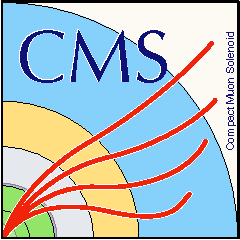
\includegraphics[width=.1\linewidth]{./cms_logo.pdf}
      };
      \node [inner sep=0pt, text width=9cm, minimum height=6cm] (cms) at (-1.64,-2.5) {
        \includegraphics[width=\textwidth]{./cms_cutaway.pdf}
      };
      \node [inner sep=0pt, text width=4cm] (text) at ($(cern) + (1.5,\the\paperheight/2)$) {
        Dummy text
      };
    \end{tikzpicture}
  % https://cds.cern.ch/record/2665537
  \end{figure}
% {\scriptsize
% L'anello di accelerazione + grande del mondo, parliamo del CMS da cui arrivano i miei dati, in cui si producono particelle in abbondanza,
%
% (foto del cern e dl cms)
%
% Del CMS mi interessa giusto introdurre il fatto che ci siano dei calorimetri perché alcuni loro parametri sono tra le features (differenze tra i calorimetri)
%
% Si produce un enorme mole di dati e per trattarli si utilizzano anche tecniche di machine learning (e così passo alla prox slide)
%
% E posso accennare molto rapidamente al Nobel di quest'anno (fallo!!)
% }
\end{frame}

\subsection{Machine Learning}
\begin{frame}{Riepilogo sul ML}
  \vspace*{-3ex}
  \begin{figure}
    \centering
    \resizebox{\linewidth}{!}{
      \begin{tikzpicture}[mindmap, outer sep=0pt,
        level 1 concept/.append style={level distance=148},
        level 2 concept/.append style={level distance=120},
        text=white,
        decoration={start radius=1cm, end radius=.5cm,amplitude=2mm,angle=30}]%,
%
        \only<-2>{
          \node [circle, minimum width=3.2cm, fill=unitocolor] (ml) at (0,0) {\huge\color{white}Machine\\[.5ex] Learning}
            child [grow=-10]
              {node [circle, minimum width=3.3cm, fill=unitograyA!60] (unsup) {\Large \!\!\!\!\!\!Unsupervised Learning}
                child [grow=-40]{ node[circle, minimum width=2.5cm, fill=unitocolor](clust)  {\normalsize Clustering}}
                child [grow=-85]{ node[circle, minimum width=2.5cm, fill=unitocolor](reduct) {\normalsize Riduzione dimensionale}}
              }
            child [grow=190] 
              {node [circle, minimum width=3.3cm, fill=unitograyA!60] (sup) {\Large Supervised Learning}
                child [grow=220]{ node[circle, minimum width=2.5cm, fill=unitocolor](classif) {\normalsize Classifi\-cazione}}
                child [grow=-95]{ node[circle, minimum width=2.5cm, fill=unitocolor](regr)    {\normalsize \!\!\!Regressione}}
          };
        }
        \only<3>{
          \node [circle, minimum width=3.2cm, fill=unitocolor] (ml) at (0,0) {\huge\color{white}Machine\\[.5ex] Learning}
            child [grow=-10]
              {node [circle, minimum width=3.3cm, fill=unitograyA!60] (unsup) {\Large \!\!\!\!\!\!Unsupervised Learning}
                child [grow=-40]{ node[circle, minimum width=2.5cm, fill=unitocolor](clust)  {\normalsize Clustering}}
                child [grow=-85]{ node[circle, minimum width=2.5cm, fill=unitocolor](reduct) {\normalsize Riduzione dimensionale}}
              }
            child [grow=190] 
              {node [circle, minimum width=3.3cm, fill=unitograyA!60] (sup) {\Large Supervised Learning}
                child [grow=220]{ node[circle, minimum width=2.5cm, fill=faircolor](classif) {\normalsize\color{black} Classifi\-cazione}}
                child [grow=-95]{ node[circle, minimum width=2.5cm, fill=unitocolor](regr)    {\normalsize \!\!\!Regressione}}
            };
          }

        \path (ml) to[circle connection bar switch color=from (unitocolor) to (unitograyA!60)] (unsup);
        \path (ml) to[circle connection bar switch color=from (unitocolor) to (unitograyA!60)] (sup);
        \path (unsup) to[circle connection bar switch color=from (unitograyA!60) to (unitocolor)] (clust);
        \path (unsup) to[circle connection bar switch color=from (unitograyA!60) to (unitocolor)] (reduct);
        \only<-2>{
          \path (sup) to[circle connection bar switch color=from (unitograyA!60) to (unitocolor)] (classif);
        }
        \only<3>{
          \path (sup) to[circle connection bar switch color=from (unitograyA!60) to (faircolor)] (classif);
        }
        \path (sup) to[circle connection bar switch color=from (unitograyA!60) to (unitocolor)] (regr);

        \node [inner sep=0pt, text width=6.5cm, minimum height=4.5cm] (nobel) at ($(ml) - (0,5.5)$) {
          \only<2->{
            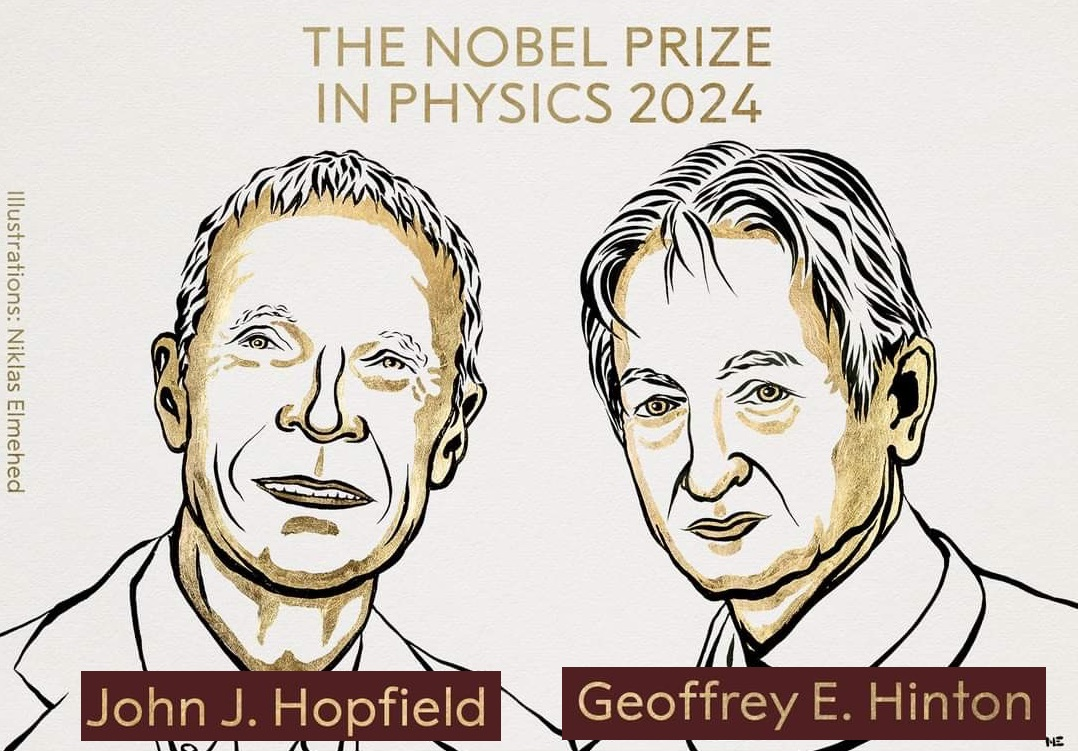
\includegraphics[width=\textwidth]{./nobel_prize.jpeg}
          }
        };
      \end{tikzpicture}
    }
  \end{figure}
%
% {\scriptsize
%   In questa slide devo far passare il concetto di labeled e unlabeled data (posso anche metterle come item)
%   Supervised eccelle nla pattern recognition, che si tratti di immagini testi o (+ vicino alla fisica) trovare mapping che siano continui o meno (nel mio caso nn lo è)
%   Qua dicendo che il mio progetto ruota attorno ad un problema di classificazione passo alla prox slide
% }
\end{frame}

\begin{frame}{Il Progetto di tesi}
% {\scriptsize
%   Che sia chiaro dove si colloca il mio progetto:
%   affrontare un problema di classificazione binaria (logistic regression), nell'ambito della Fisica delle alte energie
%
%   Immagine classica del modello std e 1 di 1 rete neurale giusto per dire rapidamente il Cosa e il Come
%
%   il mio obiettivo: allenare 1 rete che distingua al meglio tra i 2 canali di decadimento
% }
  \vspace*{-3.5ex}
  \begin{center}
    \Large
    Classificare
  \end{center}
  \vspace*{-1.5ex}
  \begin{columns}[T]
    \column{.40\linewidth}
      \begin{block}{}
        \centering%
        Bosoni elettrodeboli
      \end{block}
      \begin{figure}
        \centering
        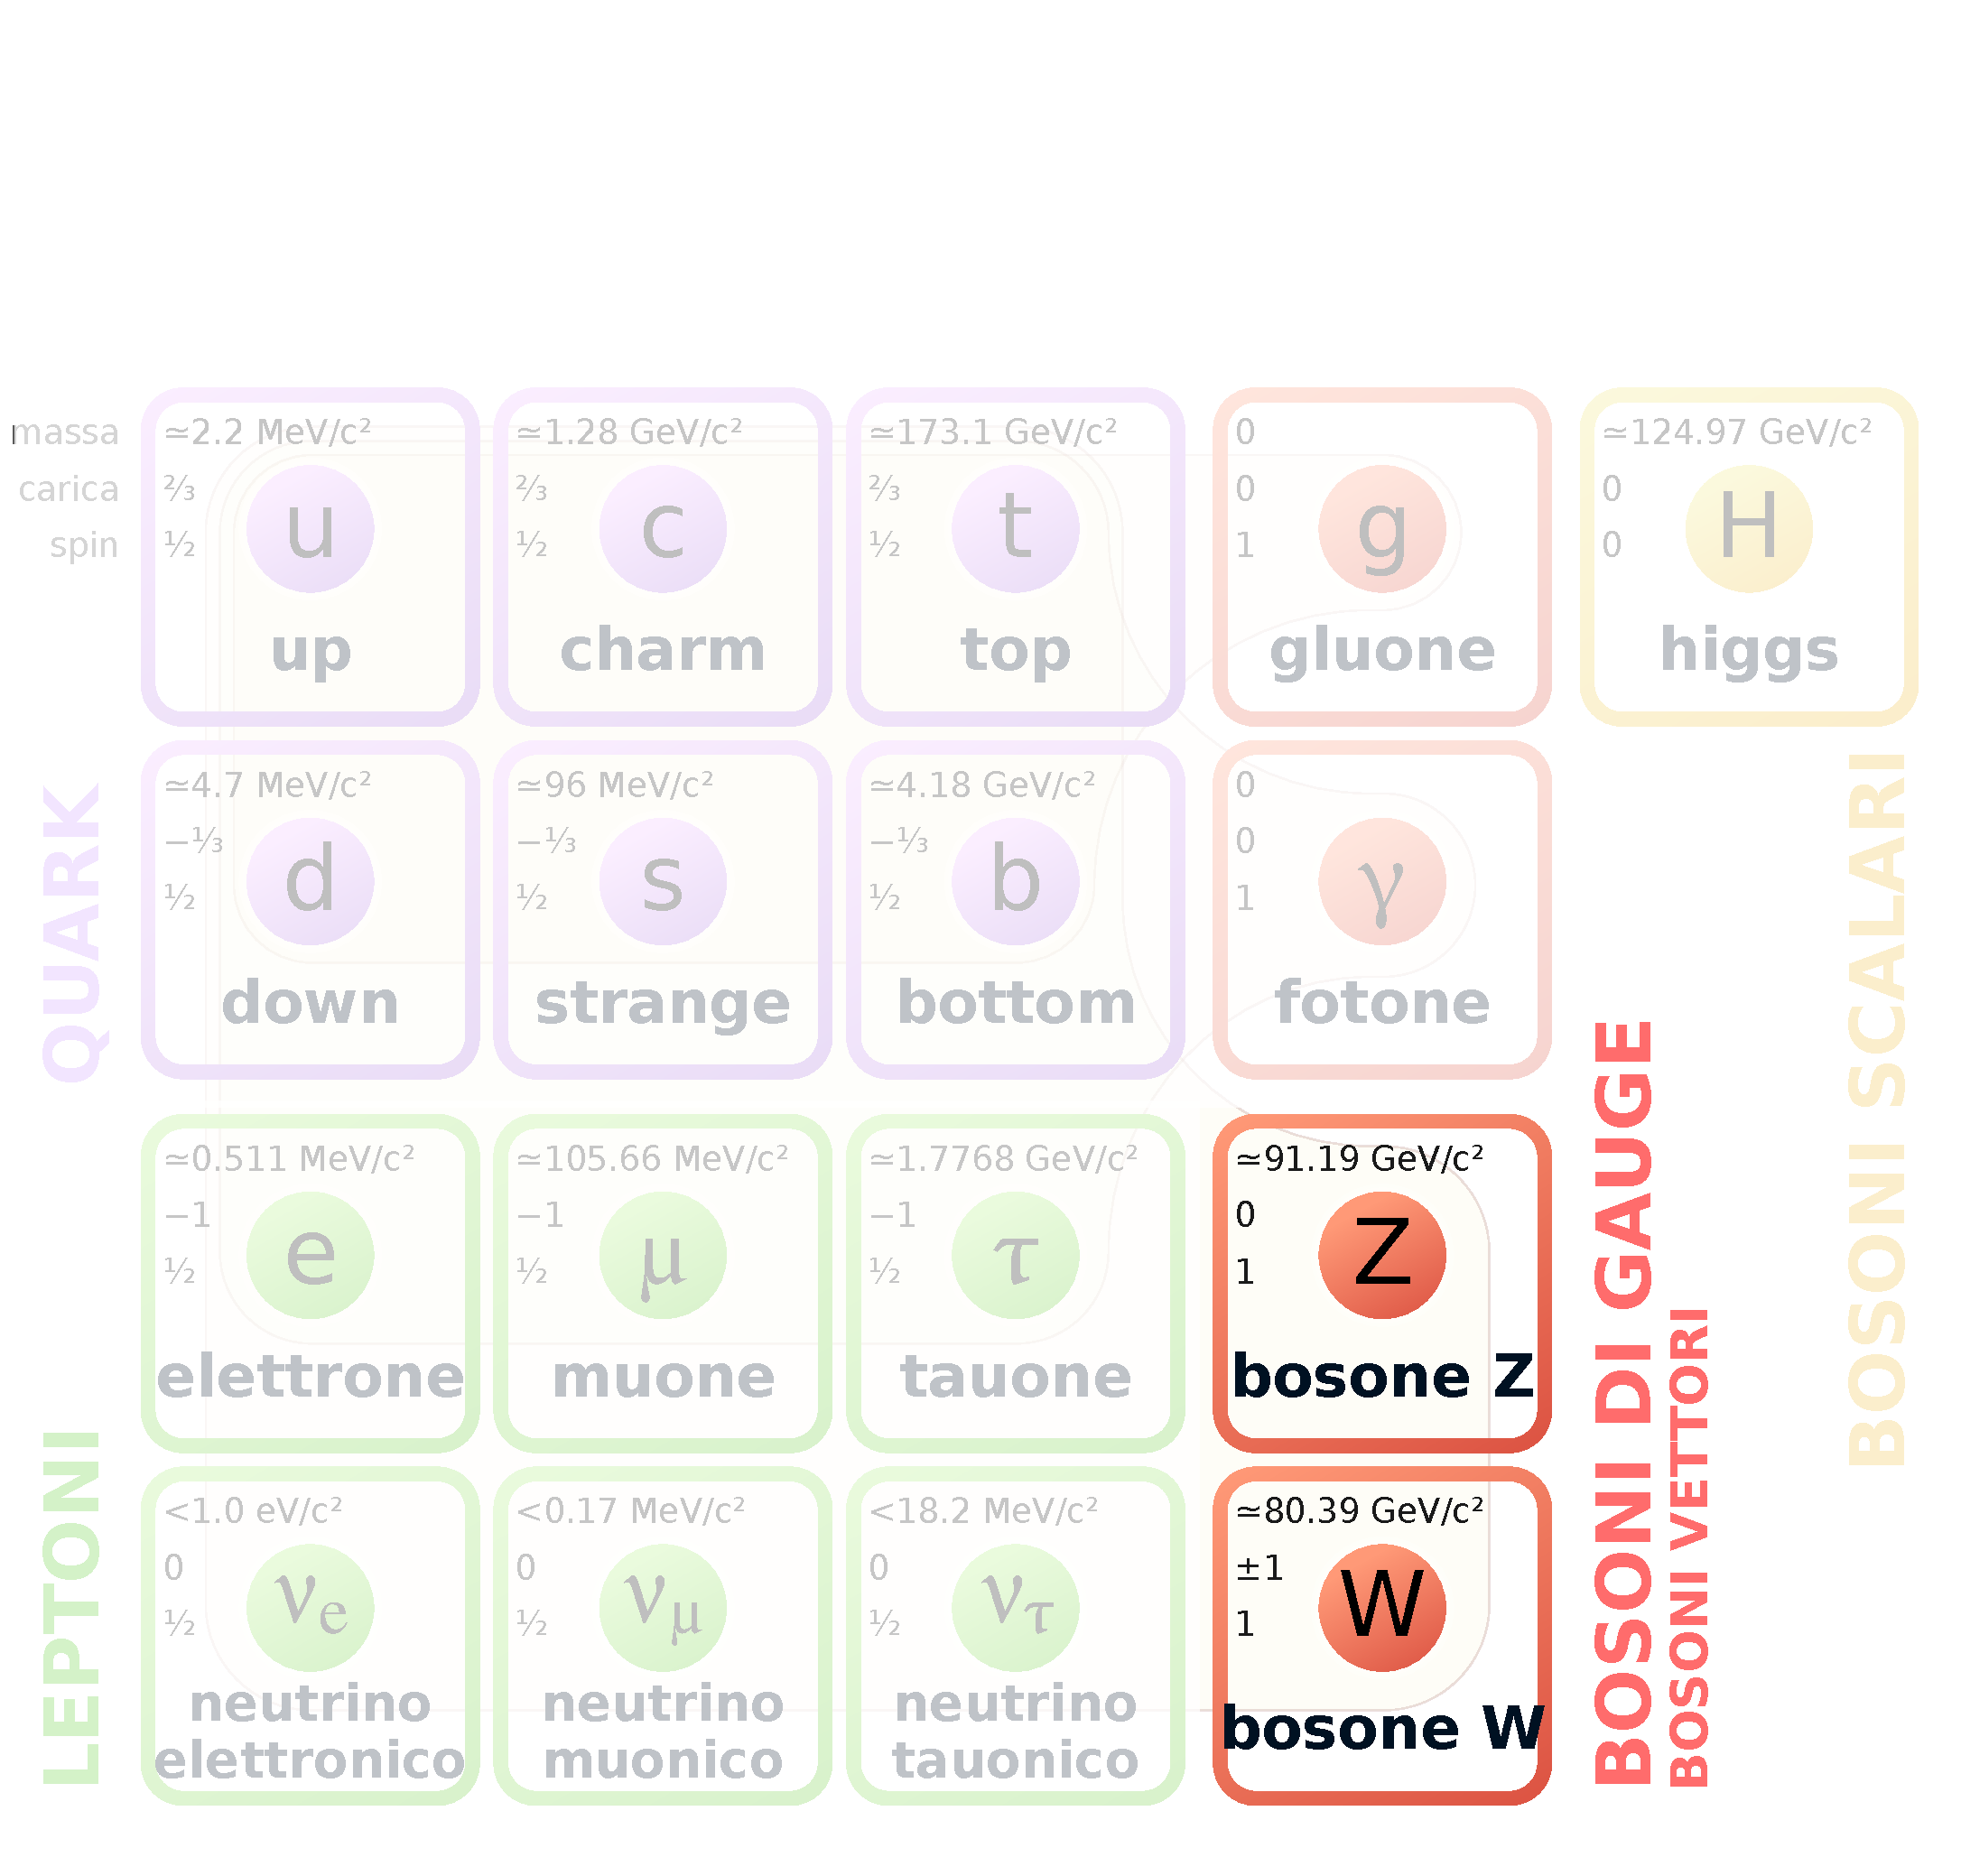
\includegraphics[width=\textwidth]{./sm_overview.pdf}
      \end{figure}

    \column{.11\linewidth}
      {
        \setbeamercolor{block body}{bg=white, fg=black}
        \begin{block}{}
          \centering\small
          con una
        \end{block}
      }
    \column{.35\linewidth}
      \begin{block}{}
        \centering
        Rete neurale
      \end{block}
      \parbox[t][][c]{\textwidth}{
        \vspace*{3ex}
        \centering
        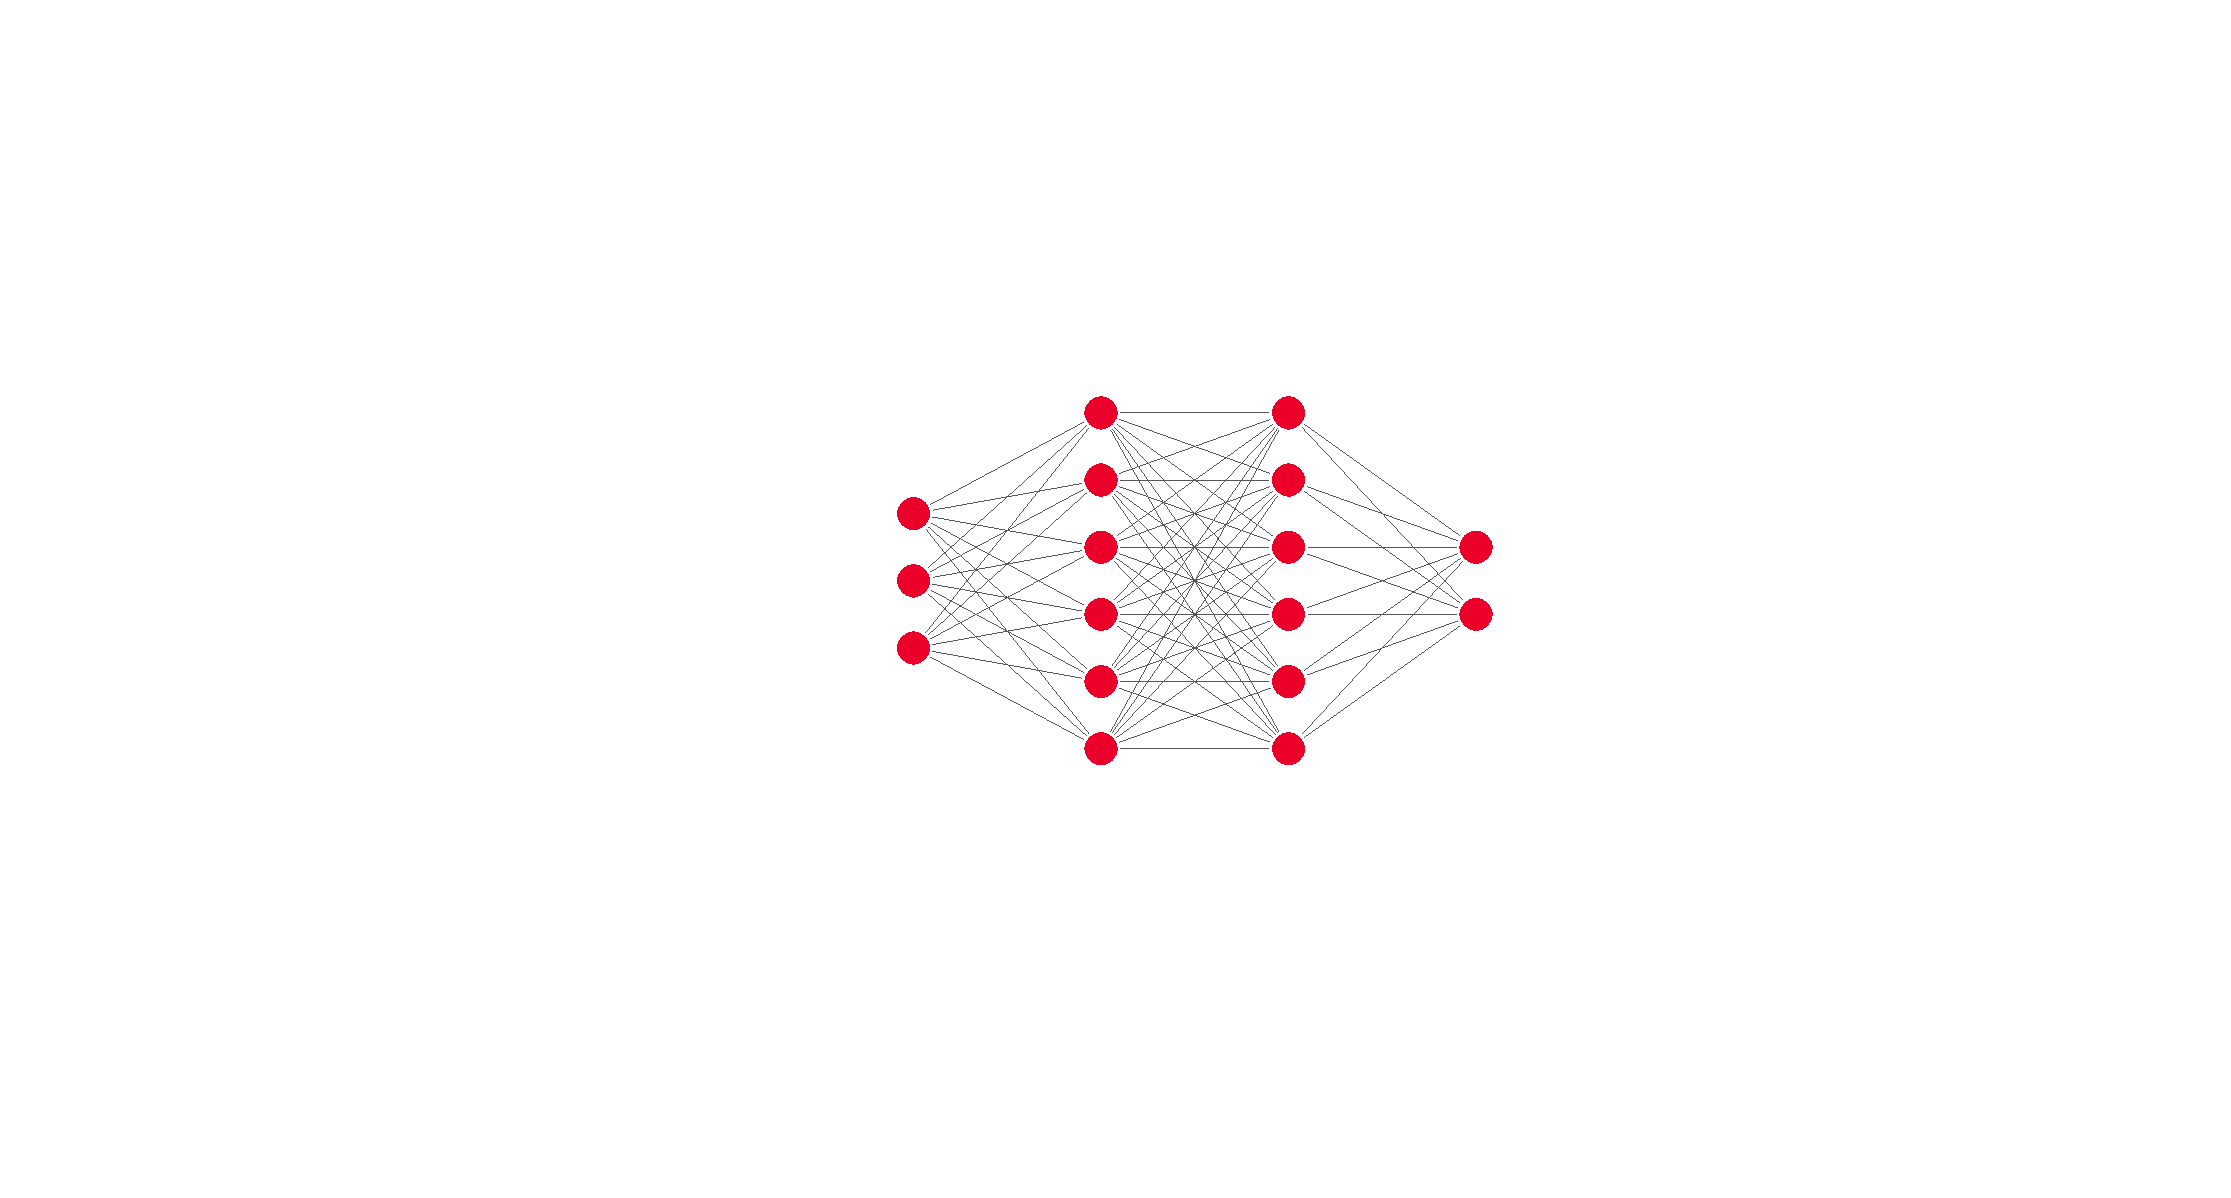
\includegraphics[width=.9\textwidth]{./nn_diagram.pdf}
      }
  \end{columns}
\end{frame}

\section{Dataset}
\begin{frame}
  \centering
  \Huge\bfseries
  Il Dataset
\end{frame}

\subsection{Decadimenti dei bosoni}
\begin{frame}{Decadimenti di $Z$ e $W$}
  qua posso mettere i diagrammi di Feynman dei decadimenti, giusto per mettere qualcosa sotto gli occhi al pubblico

  drell yann, corrente carica
% Ql è in breve la fisica del processo
\end{frame}

\begin{frame}{La struttura del dataset}
%  Diamo subito qlche dettaglio in $+$ sul dataset
  \begin{columns}
    \column{.40\linewidth}
 %    Eventi dalla Run 1 dell'LHC
      \begin{block}{}
        \centering
        Energia nel centro di massa\linebreak
        \SI{7}{\tera\electronvolt}
        \vspace*{.3ex}
      \end{block}
    % pké risale a prima dl'upgrade che lo ha portato agli odierni 13Tev nel cm
      \begin{itemize}
        \item Run 
        \item Event
        \item Variabili cinematiche dei leptoni
        \begin{itemize}
          \item momento $p_t$
          \item rapidità $\eta$
          \item angolo $\phi$
        \end{itemize}
        \item Parametri del detector iso
      \end{itemize}

    \column{.52\linewidth}
      \vspace*{6ex}
      \begin{figure}
        \centering
        \includegraphics[width=\textwidth]{./cms_event.png}
      \end{figure}
%     \vspace*{6ex}
%
  \begin{flushright}
    \scriptsize
    Datasets derived from the Run2011A:\\
    https://opendata.cern.ch/record/545
  \end{flushright}
  \vspace*{1ex}
  \end{columns}
\end{frame}

\subsection{Preprocessing}
\begin{frame}{Preprocessing}

  {\scriptsize
  Qua voglio dire che ho guardato in faccia i dati (a che scopo? cercare correlazioni evidenti e sbarazzarmi di dati che potrebbero inquinare l'allenamento dla rete), ho rimosso gli outliers e poi li ho riscalati (e dicendo qsto mi collego alla slide successiva pké la ragione dl riscalamento è strettamente legata agli algoritmi)

  Qua mostriamo sicuramente i pairplot (mi raccomando allora a inserirli riscalati!) che sono la cosa più indicativa   
  Raccontiamo la storia di correlazioni evidenti che permetterebbero una facile classificazione, nel caso $+$ semplice attraverso 1 appl lineare

  I concetti da far passare sono 2: è meglio avere 1 dataset uniforme, quindi scaliamo tutto e ci sbarazziamo degli outlier, evitare di introdurre ridondanze (ie guardare in faccia i dati con pairplot)
  }

  {\scriptsize
  la qstione dgli outlier dettagliata in slide di backup con i boxplot -> in questa maniera escono $+$ slides (e qua posso sprecarmi con il logaritmo e lo questione del'approccio scartato con le sigma)
  }
\end{frame}

\begin{frame}{Suddivisione del dataset}
  \begin{columns}
      \column{.4\linewidth}
      \begin{figure}
        \resizebox{\textwidth}{!}{
          \begin{tikzpicture}
            \coordinate (A) at (0,0);
            \coordinate (B) at (8,0); % this is the width of the rectangle
            \coordinate (C) at (8,10);
            \coordinate (D) at (0,10); % this is the height of the rectangle
            \coordinate (AB) at (6.4,0); % qsto voglio che sia a 0.8 AB
            \coordinate (AD) at (0,2); % qsto voglio che sia a 0.2 AD
            \useasboundingbox (A) rectangle (C);

            \only<1>{
              \draw [fill=unitocolor!70] (A) -- (B) -- (C) -- (D) -- (A);
              \path (4,5) node (dataset)[line width=.1cm, text width=5cm] {\begin{center}\huge\bfseries\color{white}Dataset\end{center}};
            }
            \only<2>{
              \draw [fill=unitocolor!70] (A) -- ($(AB) - (1pt,0)$) --++ (D) -- (D) -- (A);
            }
            \only<2->{
              \draw [unitograyA, fill=unitograyA] ($(AB) + (1pt,0)$) -- (B) -- (C) -- ($(AB) + (1pt,0) + (D)$);
            }
            \only<3->{
              \draw [unitocolor, fill=unitocolor!80] ($(AD) + (0,1pt)$) -- ($(AB) + (AD) + (-1pt,1pt)$) --++ ($(D) - (AD) - (0,1pt)$) -- (D) -- ($(AD) + (0,1pt)$);
              \draw [faircolor, fill=faircolor!80] (A) -- ($(AB) - (1pt,0)$) --++ ($(AD) - (0,1pt)$) -- ($(AD) - (0,1pt)$) -- (A);
            }
            % sadly the coordinates for text are hard coded :(
            \only<2->{
              \path (7.2,5.4) node (test)[line width=.1cm, text width=.4cm, minimum height=5cm] {\begin{center}\huge\bfseries\color{white}T\linebreak e\linebreak s\linebreak t\end{center}};
            }
            \only<3->{
              \path (3.2,1.4) node (val)[line width=.1cm, text width=4cm] {\begin{center}\huge\bfseries\color{black}Validation\end{center}};
              \path (3.2,5.9) node (train)[line width=.1cm, text width=3cm] {\begin{center}\huge\bfseries\color{white}Train\end{center}};
            }
          \end{tikzpicture}
        }
      \end{figure}
      \vspace*{1.5ex}

    \column{.55\linewidth}
      Bisogna evitare di insegnare alla rete il rumore statistico dei dati
      \begin{itemize}
        \item<2->Test per il genralisation check
        \item<3->Validation per valutare l'allenamento della rete
        \item<3->Train per allenare la rete
      \end{itemize}


    \end{columns}
    % e qua il collegamento con la slide successiva viene facilissimo
\end{frame}

\section{Reti Neurali}
\subsection{Architettura e principi}
\begin{frame}
  \centering
  \Huge\bfseries
  Reti Neurali
\end{frame}

\begin{frame}{L'architettura}
  \begin{figure}
    \includegraphics[width=\linewidth]{./fcn-architecture-simple.pdf}
  \end{figure}

% Qua bisogna introdurre i parametri su cui ho agito: numero di layer, nodi, attivazione, algoritmo di ottimizzazione (questo nella slide successiva)
% ricordati di specificare quand'è che la rete prende il nome di 'deep'
% E devo spiegare come funziona la questione dei parametri (pesi e bias) e dove si introduce la non linearità (attivazione)
\end{frame}

\begin{frame}{Loss function \\Algoritmi di ottimizzazione}
  \begin{columns}
    \column{.6\linewidth}
      \begin{figure}
        \centering
        \begin{tikzpicture}
          \node [line width=.04cm, inner sep=0pt, text width=\linewidth, minimum height=5cm] (landscape) at (0,0) {
            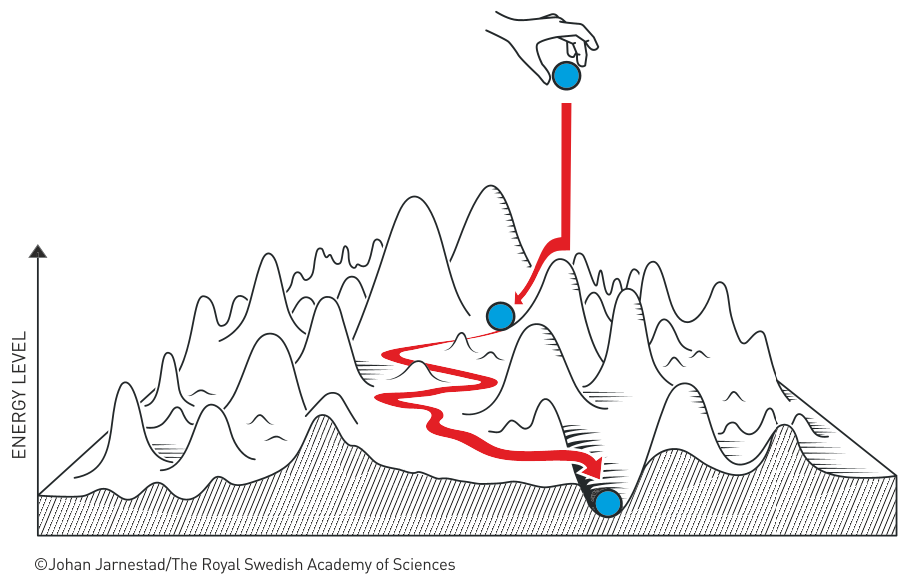
\includegraphics[width=\textwidth]{./loss_landscape.pdf}
          };
          \node [line width=.04cm, anchor=west, inner sep=0pt, text width=5cm] (loss) at ($(landscape) + (-3,3.3)$) {
            \begin{equation*}
              H(p,q) = - \sum p(x) \log q(x)
            \end{equation*}
          };
        \end{tikzpicture}
      \end{figure}
    \column{.35\linewidth}
    % \begin{equation*}
    %   H(p,q) = - \sum p(x) \log q(x)
    % \end{equation*}
      \begin{itemize}
        \item Gradient Descent
        \item RMS
        \item Adam
        \item Nadam
      \end{itemize}
  \end{columns}

  % Qsto per spiegare come funzioni la rete, nn per mostrare risultati ancora
% L'idea di 1 loss function da minimizzare (come se fosse un'energia), qsta nn è semplice da spiegare visivamente, di questa metterei proprio la formula così la commento un attimo
%
% Algoritmo (sarebbe carino accennare al learning rate e al momento e all'adattività degli algoritmi)
%
%
% Immagini di allenamenti significativi, magari anche in cui si veda l'overfitting
\end{frame}

\subsection{Risultati dell'allenamento}
\begin{frame}{Risultati}
  E qua ci va una carrellata di rock curves che può tranquillamente occupare $+$ slides, quali voglio scegliere come significative? Con algoritmi diversi e mostrando bene il test point

\end{frame}


\section{Conclusioni}
\begin{frame}{Conclusioni}
  \begin{itemize}
    \item Le reti neurali si prestano molto bene a compiti di identificazione di particelle
    \item L'allenamento è efficace perché \textbf{generalizza} al test set
    \item Ho identificato una classe di \textbf{modelli equivalenti}
  \end{itemize}
  \vspace{2ex}

  Ulteriori sviluppi: 
  \begin{itemize}
    \item combinare i dataset rimuovendo le labels per allenare una rete a distinguere i bosoni tra loro
    \item utilizzare una di queste reti come modello generativo per fare simulazioni 
  \end{itemize}
%
%   \vspace*{2ex}
    \begin{columns}
      \column{.25\linewidth}
      {
        \only<1>{\setbeamercolor{block body}{bg=white, fg=white}}
        \begin{block}{}
          \centering\vspace*{.5ex}
          \only<1>{}
          \only<2>{
            \Large\bfseries
            \color{white}
            Grazie%
          }%
        \vspace*{.5ex}
      \end{block}
      }
    \end{columns}
\end{frame}

\end{document}
